%  LaTeX support: latex@mdpi.com 
%  In case you need support, please attach all files that are necessary for compiling as well as the log file, and specify the details of your LaTeX setup (which operating system and LaTeX version / tools you are using).

%=================================================================
\documentclass[journal,article,submit,moreauthors,pdftex, applsci]{Definitions/mdpi} 

% If you would like to post an early version of this manuscript as a preprint, you may use preprint as the journal and change 'submit' to 'accept'. The document class line would be, e.g., \documentclass[preprints,article,accept,moreauthors,pdftex]{mdpi}. This is especially recommended for submission to arXiv, where line numbers should be removed before posting. For preprints.org, the editorial staff will make this change immediately prior to posting.

%----------
% submit
%----------
% The class option "submit" will be changed to "accept" by the Editorial Office when the paper is accepted. This will only make changes to the frontpage (e.g., the logo of the journal will get visible), the headings, and the copyright information. Also, line numbering will be removed. Journal info and pagination for accepted papers will also be assigned by the Editorial Office.

%------------------
% moreauthors
%------------------
% If there is only one author the class option oneauthor should be used. Otherwise use the class option moreauthors.

%=================================================================
\firstpage{1} 
\makeatletter 
\setcounter{page}{\@firstpage} 
\makeatother
\pubvolume{xx}
\issuenum{1}
\articlenumber{5}
\pubyear{2019}
\copyrightyear{2019}
%\externaleditor{Academic Editor: name}
\history{Received: date; Accepted: date; Published: date}
%\updates{yes} % If there is an update available, un-comment this line

%% MDPI internal command: uncomment if new journal that already uses continuous page numbers 
%\continuouspages{yes}

%------------------------------------------------------------------
% The following line should be uncommented if the LaTeX file is uploaded to arXiv.org
%\pdfoutput=1

%=================================================================
% Add packages and commands here. The following packages are loaded in our class file: fontenc, calc, indentfirst, fancyhdr, graphicx, lastpage, ifthen, lineno, float, amsmath, setspace, enumitem, mathpazo, booktabs, titlesec, etoolbox, amsthm, hyphenat, natbib, hyperref, footmisc, geometry, caption, url, mdframed, tabto, soul, multirow, microtype, tikz

\usepackage[single=true, macros=true, xspace=true]{acro}  % For acronyms
\usepackage{cleveref} % For references
\usepackage[squaren,Gray]{SIunits}
\usepackage{subcaption}
% \usepackage{tikz}


%=================================================================
%% Please use the following mathematics environments: Theorem, Lemma, Corollary, Proposition, Characterization, Property, Problem, Example, ExamplesandDefinitions, Hypothesis, Remark, Definition, Notation, Assumption
%% For proofs, please use the proof environment (the amsthm package is loaded by the MDPI class).

%=====================================
% INPUTS
%=====================================
%% Acronym definition example using glossaries package
%% \usepackage{acro} is required
%% 
%% For a powerful usage of the acro package look at http://tex.stackexchange.com/questions/135975/how-to-define-an-acronym-by-using-other-acronym-and-print-the-abbreviations-toge

 \DeclareAcronym{auc}{
  short = AUC,
  long =  area under the curve
}

 \DeclareAcronym{bcc}{
  short = BCC,
  long =  basal cell carcinoma
}

 \DeclareAcronym{cart}{
  short = CART,
  long =  classification and regression trees
}

\DeclareAcronym{cnn}{
  short = CNN,
  long = convolutional neural network
}

\DeclareAcronym{dej}{
  short = DEJ,
  long =  dermal-epidermal junction
}

\DeclareAcronym{ert}{
  short = ERT,
  long =  extremely randomized trees
}

\DeclareAcronym{gb}{
  short = GB,
  long = gradient boosting
}

\DeclareAcronym{ggd}{
  short = GGD,
  long = generalized Gaussian distribution
}

\DeclareAcronym{glh}{
  short = GLH,
  long = gray level histogram
}

\DeclareAcronym{glcm}{
  short = GLCM,
  long = gray level co-occurrence matrix
}

\DeclareAcronym{lm}{
  short = LM/LMM,
  long = lentigo maligna/lentigo maligna melanoma
}

\DeclareAcronym{mil}{
  short = MIL,
  long = multiple instance learning
}

\DeclareAcronym{rcm}{
  short = RCM,
  long = reflectance confocal microscopy
}

\DeclareAcronym{rf}{
  short = RF,
  long = random forest
}

\DeclareAcronym{roc}{
  short = ROC,
  long = receiver operating characteristic
}

\DeclareAcronym{sil}{
  short = SIL,
  long = Single-Instance Learning
}

\DeclareAcronym{svm}{
  short = SVM,
  long = Support Vector Machine
} 

%=================================================================
% Full title of the paper (Capitalized)
\Title{Classification of lentigo maligna at patient-level by means of reflectance confocal microscopy data}

% Author Orchid ID: enter ID or remove command
\newcommand{\orcidauthorA}{0000-0002-6449-9723} % Cendre Add \orcidA{} behind the author's name
\newcommand{\orcidauthorB}{0000-0001-9054-3719} % Mansouri
\newcommand{\orcidauthorC}{0000-0003-4479-9961} % Perrot 
\newcommand{\orcidauthorD}{0000-0002-4009-0659} % Cinotti 
\newcommand{\orcidauthorE}{0000-0003-0963-1565} % Marzani 


% Authors, for the paper (add full first names)
\Author{Romain Cendre~$^{1,*}$\orcidA{}, Alamin Mansouri~$^{1}$\orcidB{}, Jean-Luc Perrot~$^{2}$\orcidC{}, Elisa Cinotti~$^{3}$\orcidD{} and Franck Marzani~$^{1}$\orcidE{}}

% Authors, for metadata in PDF
\AuthorNames{Romain Cendre, Alamin Mansouri, Jean-Luc Perrot, Elisa Cinotti and Franck Marzani}

\address{%
$^{1}$ \quad Laboratoire ImViA (EA 7535), Université Bourgogne Franche-Comté, Dijon, France; imvia.direction@u-bourgogne.fr\\
$^{2}$ \quad Service de Dermatologie-Oncologie-Allergologie, CHU de Saint-Etienne, Saint-Etienne, France\\
$^{3}$ \quad U.O. Dermatologia, Dipartimento di Scienze Mediche, Chirurgiche e Neuroscienze, A.O.U.S. Le Scotte - Università degli Studi di Siena, Siena, Italia}

% Contact information of the corresponding author
\corres{Correspondence: romain.cendre@gmail.com}

% Abstract
\abstract{Reflectance confocal microscopy is an appropriate tool for the diagnosis of lentigo maligna. Compared with dermoscopy, this device can provide abundant information as a mosaic and/or a stack of images. In this particular context, the number of images per patient varied between 2 and 833 images and the objective, ultimately, is to be able to discern between benign and malignant classes. First, this paper evaluated classification at the image level, with the help of handcrafted methods derived from the literature and transfer learning methods. Secondly, this work proposes patient-level supervised methods based on image decisions and a comparison of these with multi-instance learning methods. In terms of image-level classification, this study achieved an F1 score of 0.83 by the use of “Inception-ResNet” architecture and SVM with a linear kernel. At the patient-level and based on “Inception-ResNet” architecture for features extraction, this study reached an F1 score of 0.83 (Sensitivity 0.88 / Specificity 0.75) with an \acs{auc} score of 0.87 for the dynamic threshold over decisions and achieve weighted F1-Score of 0.80 (Sensitivity 0.78 / Specificity 0.84) with an \acs{auc} score of 0.88 for multi-instance learning based on MI-SVM.}\par

% Keywords
\keyword{Computer-assisted diagnosis; Classification; Transfer Learning; Reflectance Confocal Microscopy; Dermatology; Lentigo}

%%%%%%%%%%%%%%%%%%%%%%%%%%%%%%%%%%%%%%%%%%
% Only for the journal Applied Sciences:
\featuredapplication{This paper focuses on improvement in patient care and it also helps practitioners optimize their dermatology services by means of computer-assisted diagnostic software using data from reflectance confocal microscopy devices.}
%%%%%%%%%%%%%%%%%%%%%%%%%%%%%%%%%%%%%%%%%%

%%%%%%%%%%%%%%%%%%%%%%%%%%%%%%%%%%%%%%%%%%
\begin{document}
%%%%%%%%%%%%%%%%%%%%%%%%%%%%%%%%%%%%%%%%%%

%=====================================
% INTRODUCTION
%=====================================
\section{Introduction}
As the incidence rate for skin cancers has steadily increased over the years, they are now the most prevalent form of human malignancy. These diseases affect people in their everyday life, as they have a pronounced social impact on the affected individuals as a result of a decrease in their quality of life as well as because they have the potential to become lethal. In addition, they have significant economic consequences, with an estimated cost of 8 billion dollars per year in the United States~\cite{Farberg2017a}, and they can stretch the ability of dermatological centers to cater to the at times overwhelming demand for screening and treatment. However, most of these repercussions can be avoided by early detection and appropriate surgeries~\cite{Farberg2017a}.\par
Currently, histological examination is the gold standard for diagnosing skin cancers in the clinical context. This process is relatively time-consuming as it requires excision of the affected area, embedding of the sample in paraffin, the generation of thin tissue sections that then need to be stained and examined by a histopathologist. However, despite its accuracy, this technique remains time-consuming, invasive, and inconvenient for doctors and patients. Consequently, several non-invasive imaging techniques have been developed to help with the classification of skin cancers, and some of these are now commonly used by dermatologists. For instance, clinical photography and dermoscopy are both examples of affordable and intuitive techniques that are presently widely used by dermatologists. Dermoscopy tends to replace clinical photography as it significantly improves the quality of the diagnoses made by experts, due largely to the acquisition of high-magnification images of the skin~\cite{Sinz2017}.\par
Research papers on dermatology nowadays tend to focus on the dermoscopy modality used to perform automatic classification of lesions. Most of them obtain acceptable results with melanocytic pathologies~\cite{Iyatomi2010}. Older methods focus on finding the most pertinent combination of preprocessing steps and handcrafted features to be used in a machine learning scheme~\cite{Rastgoo2015,Pathan2018}. By contrast, most recent methods use deep learning approaches, and they have yielded impressive results in this discipline~\cite{Esteva2017}. In this particular study, the authors used an Inception-V3 architecture pre-trained on the “ImageNet” database~\cite{Deng2008}, and they fine-tuned this model on a dataset of 129,450 clinical images containing 2,032 different skin lesions and distributed across 757 classes. They carried out the classification at different taxonomy levels, and at the first level of classification (Non-neoplastic versus Benign versus Malignant), they achieved an accuracy of 0.72$\pm$0.9\ compared to 0.66 on a subset of these data by specialists.\par
However, dermoscopy imaging devices only provide surface and chromatic information. To overcome this limitation, \ac{rcm} modality is another type of imaging technique used by dermatologists that provides high-resolution images of the skin on a micrometer scale. Furthermore, this modality can provide structural information at different depths of the skin by adjustment of the wavelength properties and the focal point~\cite{Kolm2012}. Presently, this tool has a greater diagnostic accuracy compared to dermoscopy, both for melanocytic and for non-melanocytic skin tumors~\cite{Haroon2017, Dinnes2018, Lupu2019}. Unlike the previous modalities, \ac{rcm} remains expensive, although the number of users continues to increase~\cite{Batta2015} and recent developments have led to a degree of improvement in the portability of \ac{rcm} devices~\cite{Freeman2018}.\par
By contrast, relatively fewer studies have been published on the \ac{rcm} modality by use of computer vision techniques, despite their promising results in the clinical context. The use of artificial intelligence could be particularly useful for \ac{rcm} images because their evaluation by dermatologists is time-consuming. Indeed, unlike with dermoscopy, many \ac{rcm} images need to be acquired for each skin lesion. Many studies of computer vision focus on understanding these images by predicting the position in the skin layer \cite{Somoza2014,Hames2016} using stacks of 3D data provided by this modality. A number of other studies have described the structural components of the skin~\cite{Gareau2010} and few of them have classified pathologies based on that specific modality. One of these studies~\cite{Wiltgen2008} is quite similar to the problem explored in this work, and it suggests several image descriptors for undertaking a classification task. These authors introduced two methods using frequency representation: the first one based on Fourier transform and the second one based on wavelet representation by use of Daubechies 4. The idea behind spectral representation is to extract information at different frequency levels, thereby yielding information about smoothness or complex structures inside the images, and to be consistent with rotations and translations as the pathologies are non-oriented. The second category of descriptors that they employed was based on spatial features by use of \ac{glh} and \ac{glcm} statistical descriptors. The statistical descriptors computed from \ac{glcm} had been derived from a previous work~\cite{Haralick1973}. Finally, the authors proceeded with the classification of images by using different image parts at multiple sizes and they proceeded to \ac{cart} classification. In a two-class situation, this paper reached an accuracy of 0.96 for the detection of nevi and 0.97 for melanoma pathologies by applying a wavelet extraction and \ac{cart} classification on a subpart of the 256*256 pixel images. Another paper is more relevant, as the authors followed the same purpose as this work by suggesting a way to classify solar lentigo pathologies by use of the previous wavelet decomposition, and by fitting the decomposition values to a \ac{ggd} to reduce the number of variables. They also suggested that only one variable and only one scale decomposition are relevant for solar lentigo detection. This method was applied to 45 subjects with healthy skin or solar lentigo, and it achieved a sensitivity of 0.81 and a specificity of 0.83~\cite{Halimi2017a}.\par
The scope of this work is to detect malignant tumors and particularly \ac{lm} (the most common type of facial melanoma) in \ac{rcm} images, and to help specialists reach a diagnosis based on these images at the patient-level. The previous feature extraction methods and extraction through different convolutional neural network \ac{cnn} architectures were investigated first. As wavelet decomposition and reduction through \ac{ggd}~\cite{Halimi2017a} were shown to be irrelevant in our data context~\cite{Cendre2019a}, this work did not focus on any of these methods. Comparison of several classification models on full-size images was then carried out to estimate the relevance of these methods.\par
The following parts of this paper are organized as follows. \Cref{sec:material} covers the data by proving details about their composition, the feature extraction methods implemented, and the process used to compute image-level and patient-level decisions. \Cref{sec:results} then displays all of the results and provides an analysis of them, and finally, \Cref{sec:conclusions} provides a conclusion of this work and it offers a number of perspectives.\par

%=====================================
% Materials
%=====================================
\section{Materials and Methods}
\label{sec:material}

%=====================================
% DATA
%=====================================
\subsection{Data}
\label{sec:data}
The data for this paper were originally obtained in a previous clinical study~\cite{Cinotti2018} that performed a comparison between dermoscopy and \ac{rcm} modalities in the diagnosis of benign lesions such as solar lentigo and malignant tumors by focusing essentially on \ac{lm}. These images were acquired by three specialists, experts in regard to non-invasive skin imaging tools, by use of a hand-held VivaScope® 3000 camera that uses a laser with a wavelength of \unit{830}{\nano\meter} and images to a depth of up to \unit{250}{\micro\meter}. In addition, these data included lesions that can be highly misleading for dermatology specialists.\par
Only images considered relevant for the diagnosis by two out of the three investigators were retained, at different depths of the skin: the epidermis, the \ac{dej}, and the dermis. However, most of the information was acquired at the \ac{dej}. Each \ac{rcm} image corresponded to a horizontal \unit{920}{\micro\meter} x \unit{920}{\micro\meter} section of the skin at a selected depth with a lateral resolution of \unit{1}{\micro\meter} and axial resolution of \unit{3}{\micro\meter} to \unit{5}{\micro\meter}. For specifications, these images have a spatial resolution of 1000*1000 pixels with quantification on a single 8-bits channel.\par
The \ac{rcm} device was first designed by Marvin Minksy. The principle is to emit and focus a low power laser on a specific point of the skin (see \Cref{fig:rcm} - Emission). Then the light is reflected from this point into the system optic and collected through a pinhole that allows only the light from in focus plane (see \Cref{fig:rcm} - Reception). In this situation, the illuminated point and the detector aperture have conjugate focal / confocal planes~\cite{Nehal2008a}. Different factors can affect the depth: illumination wavelength, illumination power, reflective and scattering properties of the skin.\par
\begin{figure}[h]
    \begin{center}
        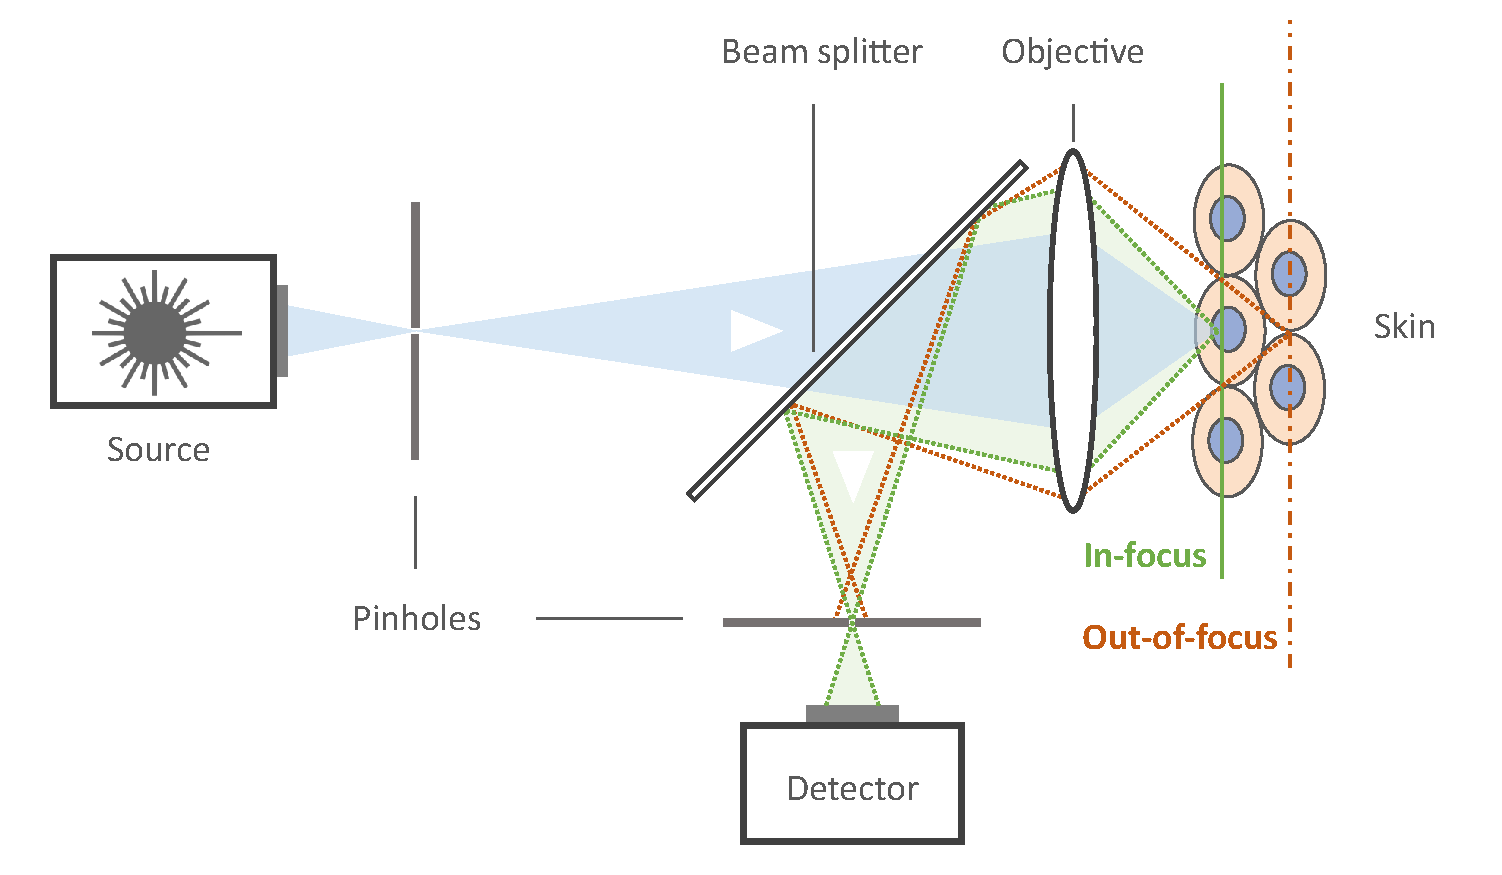
\includegraphics[width=0.7\linewidth]{Figures/RCM.pdf}
        \caption{Scheme of the \ac{rcm} principle in two steps: a low power laser is first emitted (Emission), then the reflected light is received through a pinhole (Reception).}
        \label{fig:rcm}
    \end{center} 
\end{figure}\par
Moreover, the relative position between images of a single patient was unknown, and this could not provide any further knowledge in the next part of this work. Furthermore, the metadata available regarding the age of the patients was not used as the purpose of this work was to evaluate the relevance of image classification techniques, although it was initially provided to the experts during their assessments.\par
These data included 223 patients, for a total of 7,846 RCM images, varying between 2 and 833 images per patient (with a mean of 35 and a standard deviation of 64). For each patient, the data provided a histopathology diagnosis that served as a reference basis and there was the following distribution of cases:
\begin{itemize}  
\item 135 patients had “malignant” tumors: 115 \ac{lm} and 20 \ac{bcc}.
\item 88 patients had “benign” tumors: mainly represented by solar lentigines.
\end{itemize}\par
Also, the study~\cite{Cinotti2018} evaluated 21 experts, and they achieved a mean sensitivity of 0.80 and a specificity of 0.81, with an \ac{auc} score of 0.89 for the detection of \ac{lm}.\par
In order to reduce the imbalance of the data, a further 28 additional benign tumors were provided by dermatologists, with the number of images per tumor varying between 4 and 103 images (608 images in total). These new patients were only considered for training purposes and they were not taken into account in \Cref{sec:results}.\par
In addition, these data did not provide any information regarding individual images. As these annotations were required in the next part of the work, each of these images was annotated by a specialist, with the help of a graphical interface designed for this purpose. Images with \ac{bcc} tumors were not considered as the objective is to be able to discern \ac{lm}. Whereas the patient labels were “benign” or “malignant”, some of the images could not be classified into either of these two categories because they did not contain any of these pathology signs. For this particular reason, a “healthy” label was introduced to characterize them. \Cref{fig:data} provides an overview of these different data. As this study focused only on binary classification of malignant diseases, an annotation hierarchy was defined as follows:
\begin{itemize}  
\item A “malignant” label: an image with at least some malignant tissues from \ac{lm} tumors.
\item A “benign” label: an image with no malignant tissues (either “benign” or “healthy” skin).
\end{itemize}
These annotated images amounted to 5,277 images, divided equally between men and women. The “malignant” labels accounted for 44\% of the annotated images, while the “benign” label accounted for 56\%.\par
\begin{figure}[h]
    \begin{center}
        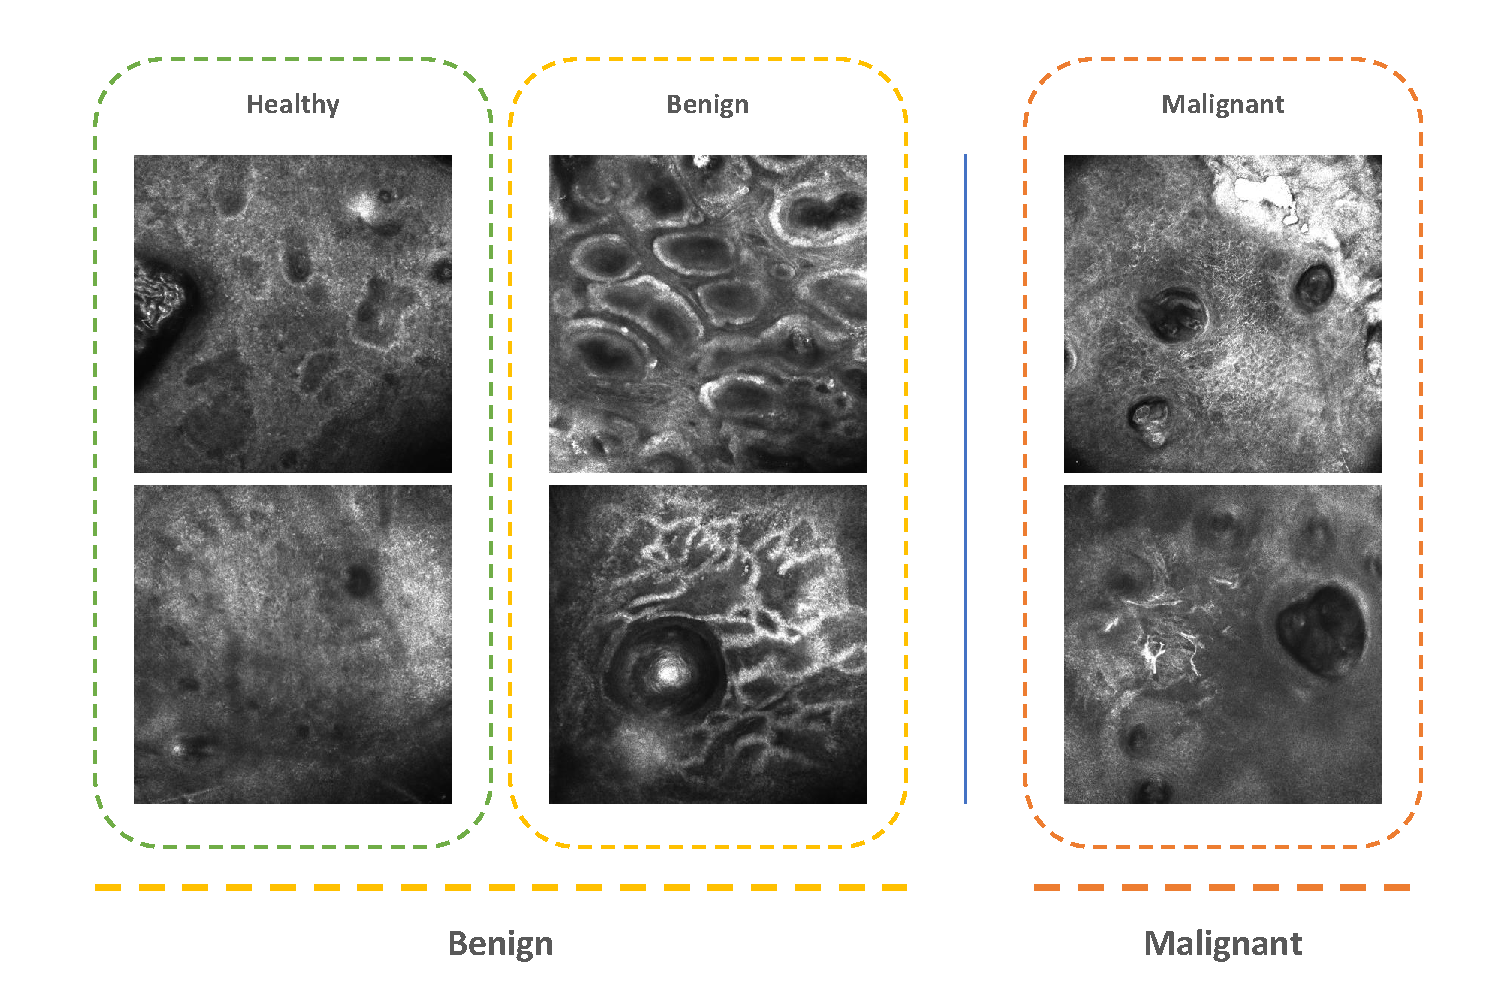
\includegraphics[width=\linewidth]{Figures/Data.pdf}
        \caption{This figure shows several examples of images related to the three different types of tissue: namely “healthy”, “benign” and “malignant”. For this work purpose, the “healthy” and “benign” labels are merged under the “benign” label.}
        \label{fig:data}
    \end{center} 
\end{figure}\par

%=====================================
% Features
%=====================================
\subsection{Feature extraction methods}
\label{sec:features}
In order to classify the data, a reduction of the image information had to be performed in a new feature space able to distinguish “malignant” from “benign” image types. According to the dermatologists, texture plays an important role in the differentiation of the tissue types. The first part of this section focuses on handcrafted feature extractors based on texture from a previous work~\cite{Wiltgen2008}. The deep extraction methods applied to this context and inspired by a previous work on dermoscopy images~\cite{Esteva2017} are then detailed. All of the feature extraction methods are listed in \Cref{tab:features_methods}, and the next parts follow this table structure.\par
\begin{table}[h]
    \centering
    \begin{tabular}{lll}
    \hline
    \textbf{Category}                   &  \textbf{Name}                & \textbf{Number of features}  \\ \hline
    \multirow{2}{*}{Spatial}            &  Haralick                     & 12                        \\ \cline{2-3} 
                                        &  \ac{glh}+\ac{glcm}           & 17                        \\ \hline 
    \multirow{2}{*}{Frequency}          &  Fourier                      & 38                        \\ \cline{2-3} 
                                        &  Wavelet                      & 39                        \\ \hline
    \multirow{5}{*}{Transfer Learning}  &  VGG-16                       & 512                       \\ \cline{2-3} 
                                        &  Inception-V3                 & 2048                      \\ \cline{2-3} 
                                        &  ResNet                       & 2048                      \\ \cline{2-3} 
                                        &  Inception-ResNet             & 1536                      \\ \hline
    Fine Tuning                         &  ResNet                       & 2048                      \\ \hline
    \end{tabular}
    \caption{The list of all of the feature extraction methods performed in this paper and their associated extracted number of features.}
    \label{tab:features_methods}
\end{table}\par
The “Spatial” extraction methods were based on spatial patterns of pixels, by use of \ac{glh} and \ac{glcm}. The method called “Haralick” refers to previous work based on texture features [18] and it uses the \ac{glcm} concept by computation of the twelve statistical characteristics listed in \Cref{tab:histogram_features} - \ac{glcm} Features column. These characteristics were extracted along horizontal, vertical, and two diagonals. A mean was computed along these axes as the tissues are not oriented in space, and to reduce the number of features. A second method from a previous work~\cite{Wiltgen2008}, called “\ac{glh}+\ac{glcm}” in this paper, expanded the first twelve initial characteristics of Haralick and it added five others based on \ac{glh}. In total, 17 features were extracted for each image, and all of the statistical properties extracted are listed in \Cref{tab:histogram_features}. The Haralick features extraction was performed using the “Mahotas” library~\cite{coelho2012mahotas} and histogram feature extraction was computed with help from the “Scipy” library~\cite{Jones2001}.\par
\begin{table}[h]
    \centering
    \begin{tabular}{ll}
        \hline
        \textbf{\ac{glcm} Features}& \textbf{\ac{glh} Features}     \\ \hline
        Angular Second Moment      & Mean value                     \\
        Difference Moment          & Mean square deviation          \\
        Correlation                & Skewness                       \\
        Sum of Squares             & Kurtosis                       \\
        Inverse Difference Moment  & Entropy                        \\     
        Summed Average             &                                \\    
        Sum Variance               &                                \\    
        Entropy                    &                                \\    
        Sum Entropy                &                                \\    
        Difference Entropy         &                                \\    
        Measure of Correlation 1   &                                \\  
        Measure of Correlation 2   &                                \\ 
    \end{tabular}
    \caption{The statistical measures derived from \ac{glcm} and \ac{glh}, respectively, and extracted in order to perform “Spatial” extraction methods.}
    \label{tab:histogram_features}
\end{table}\par
A second category of extraction methods, called “Frequency”, refers to a set of methods based on frequency approaches. The first method of this category is called “Fourier” and is based on Fourier transform. The main idea is to provide different levels of information as high frequency refers to high-contrast parts and low frequencies to homogeneous areas in the image. As the spectrum is symmetrical around the origin, only half of this spectrum was considered for the sake of computational efficiency. Then, a mean value was computed for all of the coefficients located at the same radial distance from the origin, at 22 different radius sizes between 0 and the diagonal size of the image. A previous paper~\cite{Smach2008a} has also shown the relevance of this method in the context of textural images. Finally, 16 constant directions were taken from the origin of the power spectrum, and a mean value was computed for each of them~\cite{Wiltgen2008}. The second method of this category is called “Wavelet” in this work and is based on Wavelet transform by use of a decomposition based on a Daubechies 4 that provides quite fine localization properties~\cite{Wiltgen2008}. This decomposition was made at five scales, and only the four last scales were considered to compute coefficients. For each of them, three statistical measures were computed: the standard deviation, the energy, and the entropy.\par
% \begin{figure}[h]
%     \begin{center}
%         \begin{tikzpicture}[scale=1.2]
%             \node[] at (-2, 0) {a)};
%             \begin{scope}
%                 \clip (-1.5, -1.5) rectangle (1.5, 1.5);
%                 \foreach \cRadius in {1, ..., 22}
%                     \pgfmathsetmacro\cColor{\cRadius/22*100} %22-22}
%                     \draw[red!\cColor!blue, densely dotted] (0, 0) circle (0.02+\cRadius*0.1); 
                    
%                 \fill[blue!20] (-1.5, -1.5) rectangle (0, 1.5);
%                 \draw[blue!60, ultra thick] (-1.5, -1.5) rectangle (1.5, 1.5);
%             \end{scope}
%         \end{tikzpicture}
%         \qquad
%         \begin{tikzpicture}[scale=1.2]
%             \begin{scope}
%                 \clip (-1.5, -1.5) rectangle (1.5, 1.5);
%                 \foreach \cAngle in {1, ..., 16}
%                     \pgfmathsetmacro\cColor{\cAngle/16*100}
%                     \draw[red!\cColor!blue, densely dotted] (0, 0) -- (\cAngle* 180 / 15 -102:3); 
%                 \fill[blue!20] (-1.5, -1.5) rectangle (0, 1.5);
%                 \draw[blue!60, ultra thick] (-1.5, -1.5) rectangle (1.5, 1.5);
%             \end{scope}
%         \end{tikzpicture}
%         \qquad
%         \vrule
%         \qquad
%         \begin{tikzpicture}[scale=1.2]
%             \node[] at (-2, 0) {b)};
%             % First level
%             \draw[blue!60, thick] (-1.5, -1.5) rectangle (0, 0);
%             \draw[blue!60, thick] (0, -1.5) rectangle (1.5, 0);
%             \draw[blue!60, thick] (0, 0) rectangle (1.5, 1.5);
%             % Second level
%             \filldraw[blue!60, fill=blue!5, thick] (-1.5, 0) rectangle (-0.75, 0.75) node[pos=.5] {15};
%             \filldraw[blue!60, fill=blue!5, thick] (-0.75, 0) rectangle (0, 0.75) node[pos=.5] {14};
%             \filldraw[blue!60, fill=blue!5, thick] (-0.75, 0.75) rectangle (0, 1.5) node[pos=.5] {13};
%             % Third level
%             \filldraw[blue!60, fill=blue!15, thick] (-1.5, 0.75) rectangle (-1.5+0.375, 0.75+0.375) node[pos=.5] {12};
%             \filldraw[blue!60, fill=blue!15, thick] (-1.5+0.375, 0.75) rectangle (-1.5+0.75, 0.75+0.375) node[pos=.5] {11};
%             \filldraw[blue!60, fill=blue!15, thick] (-1.5+0.375, 0.75+0.375) rectangle (-1.5+0.75, 0.75+0.75) node[pos=.5] {10};
%             \filldraw[blue!60, fill=blue!35, thick] (-1.5, 0.75+0.375) rectangle (-1.5+0.375, 0.75+0.75) node[pos=.5] {...};
%         \end{tikzpicture}
%     \end{center}
%     \caption{On the left, the feature extraction process by Fourier transform, first by drawing circular masks (22 in total) and then taking directions (16 in total). On the right, the wavelet decomposition described with an applied measure of 0-16.}
%     \label{fig:handcrafted}
% \end{figure}\par
The third category of methods investigated was in regard to deep learning methods and more specifically in regard to \ac{cnn}, which are known to be well-suited methods for image classification, thanks to robust feature patterns~\cite{Pathan2018}. Many architectures were used to address ImageNet challenges, and their associated performances were analyzed~\cite{Canziani2016}. Instead of training this network from scratch, as we have data constraints and also computational constraints, we choose a Domain Adaptation approach for these models. Most of the papers to date have dealt with \ac{cnn} trained on ImageNet~\cite{Deng2008}, as this database contains thousands of classes and more than 14 million images, meaning that the extracted features from these networks can be used in various fields. As discussed by~\cite{Litjens2017}, Inception-V3 architecture pre-trained on ImageNet is thought to be the most relevant for medical applications. As \ac{rcm} images can have various forms and can contain specifics details compared to other image modalities, this research compares the most well known \ac{cnn} architectures: VGG-16~\cite{Simonyan2014}, Inception-V3~\cite{Szegedy2015}, ResNet~\cite{He2016} and Inception-ResNet~\cite{Szegedy2017}, with accuracies of 0.71, 0.76, 0.78, and 0.80, respectively, on the ImageNet database~\cite{Canziani2016}. This method involves use of Transfer Learning, by removing the last layers devoted to the classification task, in order to obtain a new representation of the image data as features. Furthermore, in order to reduce the number of features provided by the previous step, a global pooling layer based on the maximum of each activation layer was performed. For convenience, this whole method is called “Transfer Learning” in the next paragraphs and the names of the respective networks are used. The \ac{cnn} computation was implemented using the “Keras” library~\cite{chollet2015keras}.\par

%=====================================
% IMAGE LEVEL
%=====================================
\subsection{Image-level decision}
\label{sec:image_decision}
The image-level decision was the first level of classification achieved in this study, whereby the image classification must be carried out according to the two classes “malignant”, as the positive class, and “benign”. In order to satisfy this objective, the process consisted of using the image as a single instance that has several discriminant characteristics and sufficient information to allow its classification. As formulated by~\cite{foulds_frank_2010}, such a problem can be set as a pair {X|y}, in which \(X=\{x_1,x_2,\ldots,x_n\}\) is a vector characteristic for which \(n\) is the number of features and \(y\) the associated label. The task consisted of finding the existing relationship between \(X\) and \(y\), using a classification process.\par 
To achieve this task, an extraction method (see \Cref{sec:features}) was applied to the images, depending on the currently evaluated method. The features were then normalized based on a standard score computation to make the classification task more accurate and robust~\cite{Graf2001}. This scaling was computed by subtracting the mean and then dividing by the standard deviation. The schematic outline in \Cref{fig:image_process} provides an overview of this process.\par
\begin{figure}[h]
    \begin{center}
        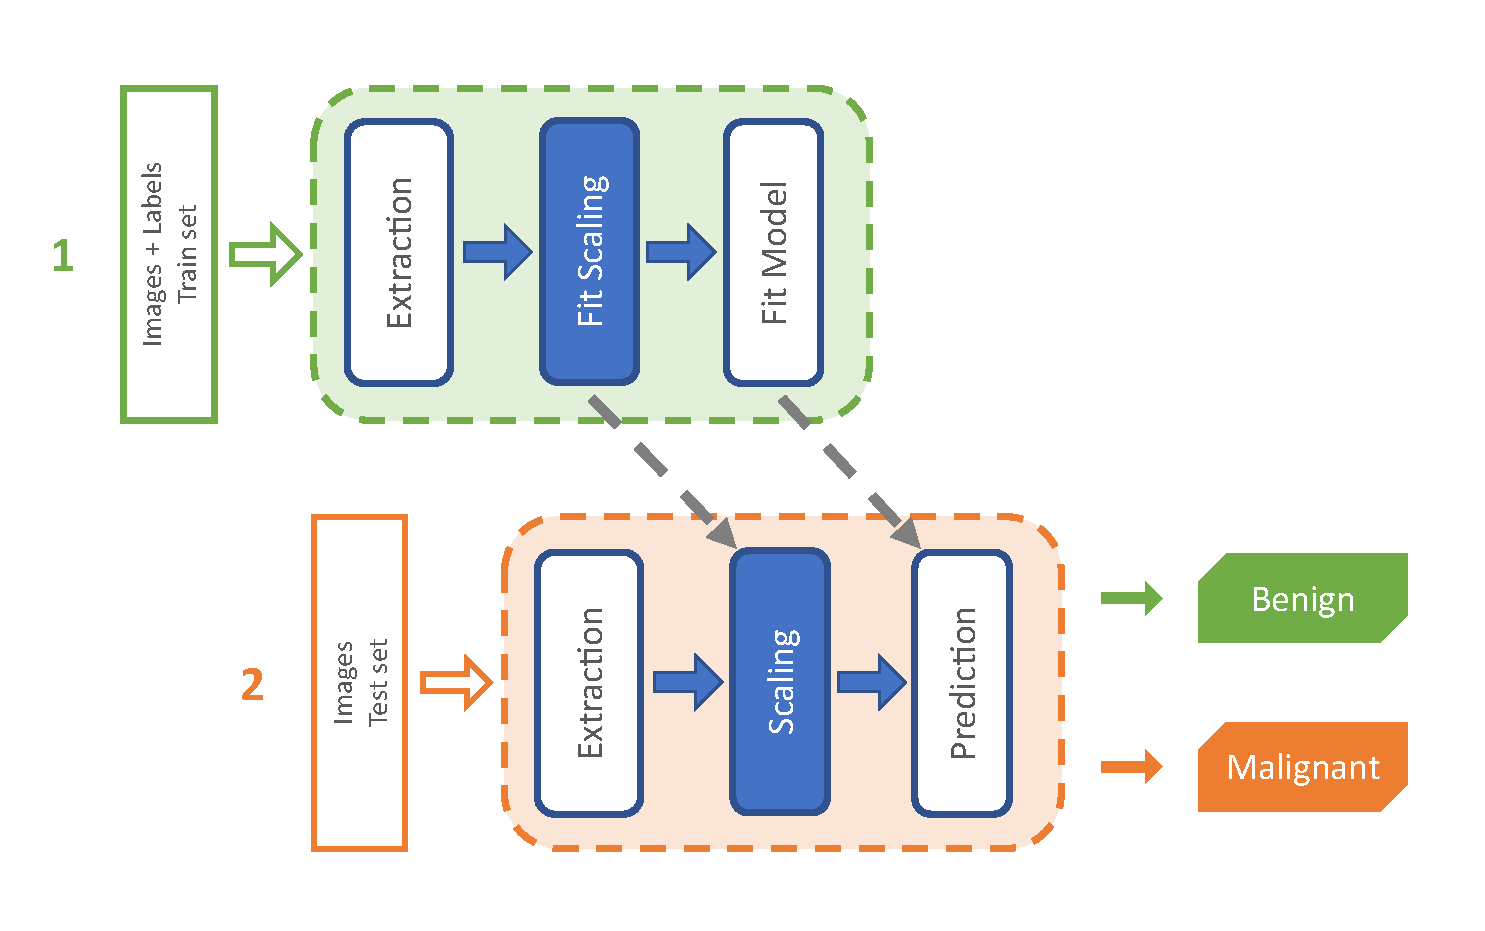
\includegraphics[width=0.8\linewidth]{Figures/Process_Image.pdf}
        \caption{The classification process performed on the \ac{rcm} images. The “Extraction” box refers to one of the Feature Extraction methods mentioned in \Cref{sec:features}. The “Fit Model” and “Prediction” boxes are related to the training and inference steps, respectively, of one of the trained and inferred models discussed in \Cref{sec:image_decision}. The testing set was predicted based on two classes: “benign” and “malignant”}
        \label{fig:image_process}
    \end{center} 
\end{figure}\par
Finally, the classification was performed on scaled features using different models. In a first stage, \ac{cart} were investigated as in a previous study in the same data context~\cite{Wiltgen2008}. In a second stage, as our number of features can be huge due to Transfer Learning methods, \ac{ert} models were also used as an extension of \ac{cart}~\cite{Geurts2006}. Lastly, \ac{svm} models were evaluated that are known to be suitable in multiples contexts~\cite{Smach2008a,Kose2016b}. As the relationship between the features and the expected outputs can be complex, \ac{svm} models were compared over linear and RBF kernels.\par
In addition, to provide the best performance with each of these models, a search in regard to their optimum hyperparameters was carried out (see \cref{tab:image_hyperparameters}).\par
\begin{table}[]
    \centering
    \begin{tabular}{lll}
    \textbf{Name}                   & \textbf{Parameter}& \textbf{Values}               \\ \hline
    \multirow{2}{*}{\ac{cart}}      & Maximum depth     & [3, $\infty$]                 \\ \cline{2-3}
                                    & Criterion         & [Gini, Entropy]               \\ \hline 
    \multirow{2}{*}{\ac{ert}}       & Maximum depth     & [3, $\infty$]                 \\ \cline{2-3}
                                    & Criterion         & [Gini, Entropy]               \\ \hline 
    \ac{svm} Linear                 & C                 & [0.01, 0.1, 1, 10, 100, 1000] \\ \hline
    \multirow{2}{*}{\ac{svm} RBF}   & C                 & [0.01, 0.1, 1, 10, 100, 1000] \\ \cline{2-3}
                                    & Gamma             & [0.01, 0.1, 1, 10, 100, 1000] \\ \hline 
    \end{tabular}    
    \caption{List of all of the classification models performed in this study and their referring evaluated hyper-parameters.}
    \label{tab:image_hyperparameters}
\end{table}\par


%=====================================
% PATIENT LEVEL
%=====================================
\subsection{Patient-level decision}
\label{sec:patient_decision}
This part relates to different ways to achieve classification at the patient-level based on the same two categories: “malignant”, as the positive class, and “benign”. With this assumption, a patient should be considered “malignant” if at least one image is considered to be “malignant”. Additionally, this part needs to consider the varying number of samples per patient (as a reminder, the number of instances per patient can vary between 2 and 833 images).\par
In order to achieve this, the best combination of the feature extraction method and the classification model from \Cref{sec:image_decision} was used. The classification model provided two types of information for each image: the score was based on prediction probabilities and the decision (i.e., the class that achieved the best probability). In both cases, due to the varying number of images per patient, the information needs to be transformed into constant-size matrices to make a decision for existing and for new patients. At the score level, the structure was composed of patients, images, and scores of classes and transformed into a new matrix of size P*C, where P is the number of patients and C is the number of classes. A dynamic threshold was then used to adjust the positive class that maximizes the chosen metric. Multiple strategies can be used to achieve this:
\begin{itemize}
\item Mean - allows the contribution of each instance on the patient to be retained
\item Maximum – retention of the best confidence prediction as the trusted one.
\end{itemize}
At the decision level, the structure was composed by structure, combining patients, images, and scores of classes and transformed into a new matrix of size P*C, where P is the number of patients and C is the number of classes. Also, C refers to the probability vector of each decision between 0 and 1.
\begin{itemize}
\item At Least One - at least one positive decision to consider as positive (initial assumption)
\item Dynamic - find a dynamic threshold that minimizes false-positive decisions.
\end{itemize}
A global overview of the processing scheme of this method is presented in \Cref{fig:decision_process}.
\begin{figure}[h]
    \begin{center}
        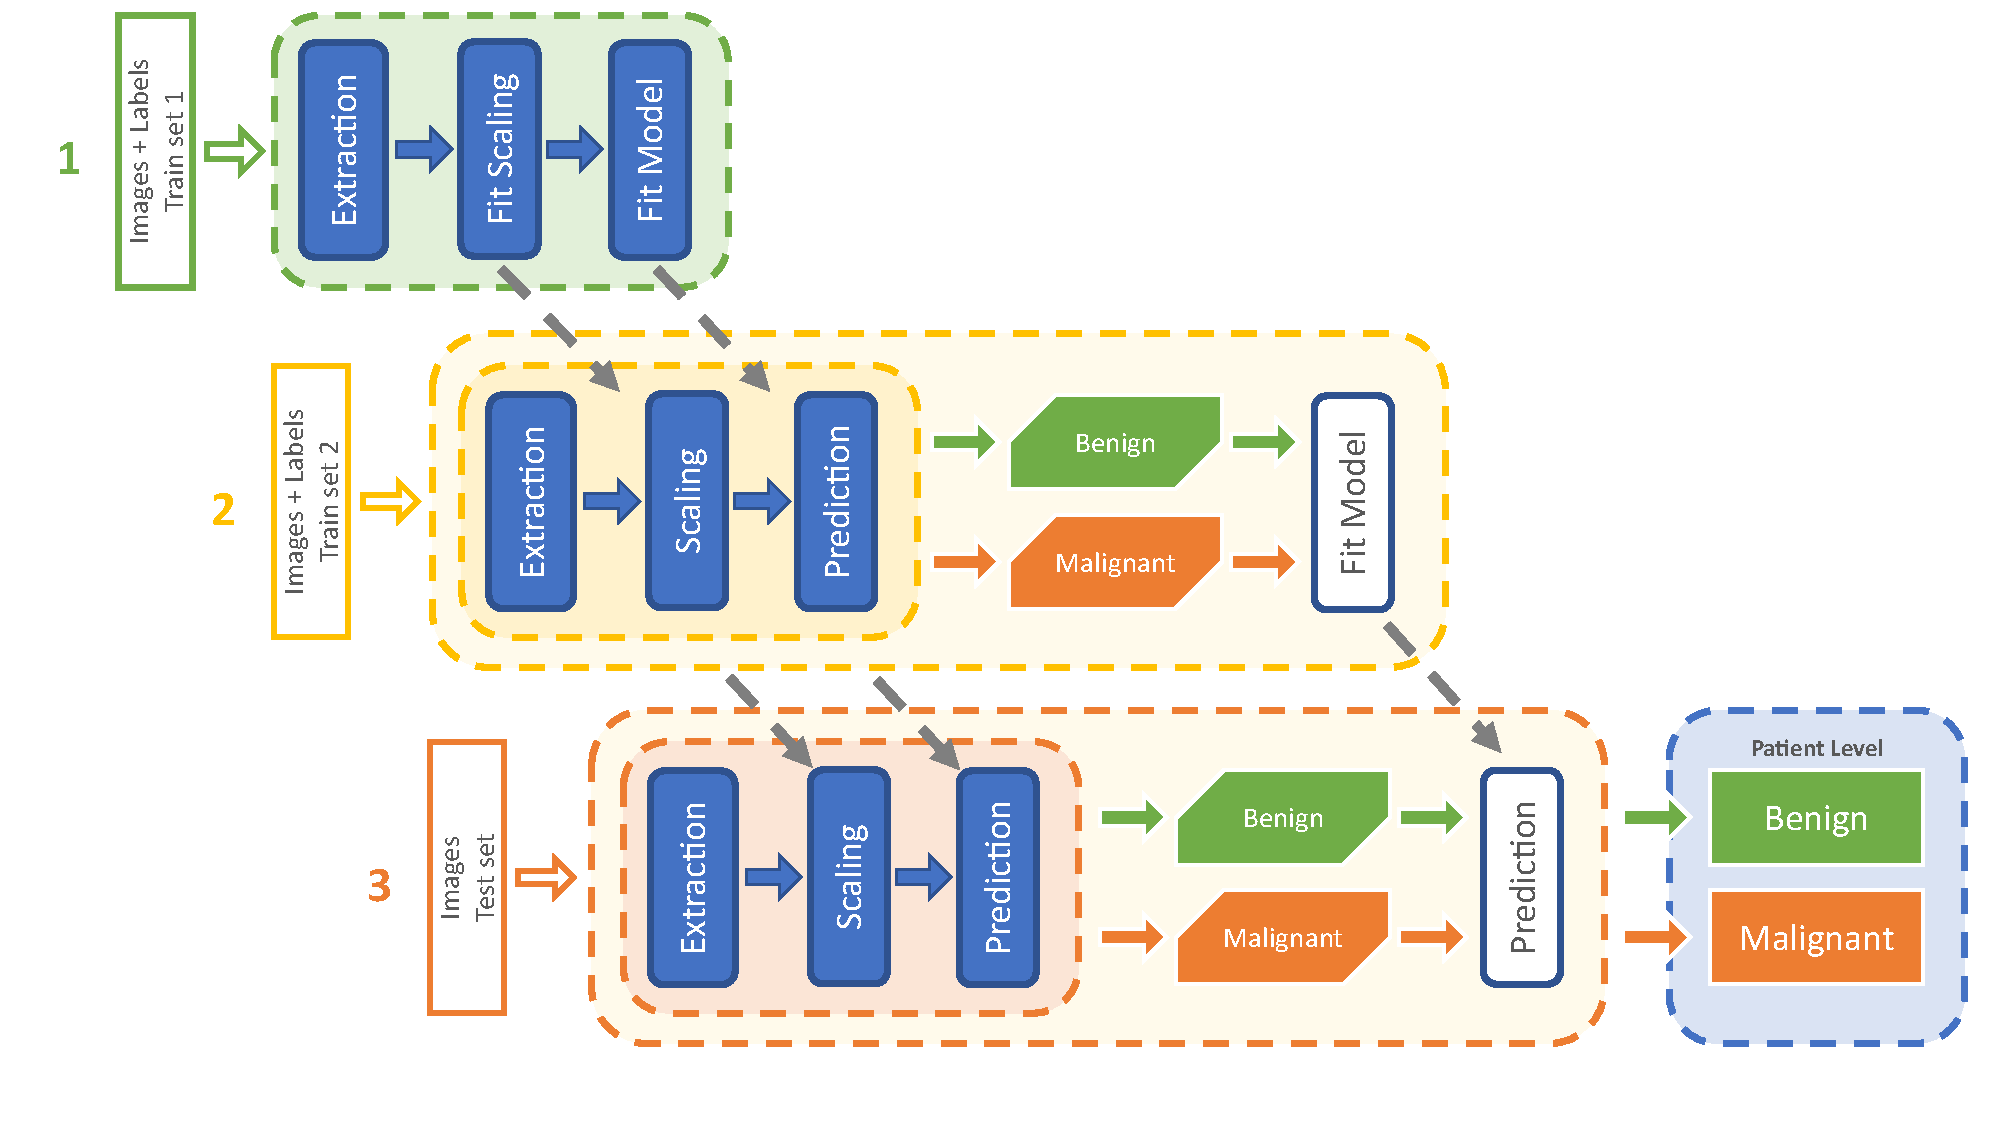
\includegraphics[width=\linewidth]{Figures/Process_Decision.pdf}
        \caption{The classification process performed on \ac{rcm} patients in which the first part of the process remained the same as in \cref{sec:image_decision}. The “Fit Model” and “Prediction” boxes refer to the decision and score level methods discussed in \Cref{sec:patient_decision}. The testing set was predicted for the patients based on “benign” and “malignant” classes.}
        \label{fig:decision_process}
    \end{center} 
\end{figure}\par
In a second stage, a number of \ac{mil} concepts are implemented in this part, as they fit the issue at hand: a patient is constitutive of several instances (consider it as a bag) and a positive instance assumes that the patient should be positive. Furthermore, only the patient label is known, and the annotation step of individual images is time-consuming. Such a problem can be set as a pair\(\{X|y\}\), in which \(X=\{X^1,X^2,\ldots,X^b\}\) is a bag containing \(b\) instances and each \(X^b\) formulated as follows: \(X^b=\{x^b_1,x^b_2,\ldots,x^b_n\}\), in which \(n\) is the number of features and \(y\) is the patient label~\cite{foulds_frank_2010}. Two ideas are developed regarding this context in the paragraphs that follow. In a first stage, a \ac{sil} classification is used in which a bag is considered as negative if all of the instances are considered to be negative, and positive if at least one of the instances has a positive label that fits our initial formulation of the patient label. In a second stage, the MI-SVM are an extension of \ac{svm} upon \ac{mil} theory and are employed in these due to the results of \Cref{sec:image_decision}. These experiments are configured to function with a linear kernel due to the observation made by the experiments of \Cref{sec:image_decision}. In this part, the experiments were implemented using the “MISVM” library~\cite{Doran2014}.\par
In addition, to provide the best performance on each of these models, a search for their optimal hyper-parameters was carried out (see \cref{tab:patient_hyperparameters}).\par
\begin{table}[]
    \centering
    \begin{tabular}{llll}
    \textbf{Category}               & \textbf{Name}     & \textbf{Parameter}& \textbf{Values}                                   \\ \hline
    \multirow{2}{*}{Score}          & Mean              & \multirow{2}{*}{-}& \multirow{2}{*}{[]}                               \\ \cline{2-2}
                                    & Maximum           &                   &                                                   \\ \hline 
    \multirow{2}{*}{Decision}       & At Least One      & \multirow{2}{*}{-}& \multirow{2}{*}{[]}                               \\ \cline{2-2}
                                    & Dynamic           &                   &                                                   \\ \hline 
    \multirow{2}{*}{\ac{mil}}       & \ac{sil}          & \multirow{2}{*}{C}& \multirow{2}{*}{[0.01, 0.1, 1, 10, 100, 1000]}    \\ \cline{2-2}
                                    & MI-SVM            &                   &                                                   \\ \hline 
    \end{tabular}    
    \caption{List of all of the classification models and referring evaluated hyper-parameters.}
    \label{tab:patient_hyperparameters}
\end{table}
\par


%=====================================
% RESULTS
%=====================================
\section{Results}
\label{sec:results}

\subsection{Validation and evaluation metric}
The validation protocol remains the same for each of these experiments, based on a nested cross-validation that is known to be less biased than a simple cross-validation scheme~\cite{Cawley2010}. This process allows 1) cross-validation of hyper-parameters and 2) objective evaluation of the prediction models. Each of the cross-validation steps is based on a K-fold strategy with a $k$ value of 4 on the testing loop and 2 on the validation loop. Also, each time, the patients are separated and balanced as best as possible based on the image labels. In order to achieve an objective evaluation, each data cluster remains the same for the experiments in a given section (refer to \cref{sec:image_decision} and \cref{sec:patient_decision}). Moreover, each experiment is validated and evaluated using an F1 score metric, as it is statistically suitable for unbalanced populations compared to an accuracy metric, and it represents in a single value recall and precision information. In addition, a standard deviation is computed to achieve an analysis of the stability of models along the nested cross-validation. For this purpose, we used the “Scikit Learn” library for Machine Learning classification, validation, and metric~\cite{pedregosa2011scikit}.\par
\subsection{Experiments and Discussion}
The results of \Cref{sec:image_decision} regarding image-level decisions were performed only on the labeled images and are listed in \cref{tab:image_results}. The most suitable handcrafted extraction method was based on the “Wavelet” method combined with the Linear \ac{svm} model, and it reached an F1 score of 0.74 with a quite stable performance of 0.04. In general, all of the handcrafted methods performed in a quite similar and stable way, varying from 0.69 to 0.74 for the F1 score and 0.03 to 0.06 for the deviation. In addition, the Transfer Learning-based feature extraction reached higher scores with the Linear \ac{svm} model, in particular with the “Inception-ResNet” architecture, which achieved a weighted F1 score of 0.83 with a deviation of 0.04. With this same model, the Transfer Learning feature extraction methods varied from 0.77 to 0.83, with a deviation range from 0.02 to 0.04. By contrast, all of these architectures performed poorly in the RBF \ac{svm} model, but this can be explained by an excessive number of features that resulted in overfitting despite the cross-validation of hyper-parameter “C”. The “VGG-16” architecture performed better with only 512 features than the remaining architectures providing 1,536 or 2,048 features. For the classification model based on Trees, no such difference was seen between \ac{cart} and \ac{ert} on the handcrafted methods, but a notable difference was found when using the Transfer Learning extraction method. This can be due to the huge number of features related to the RBF \ac{svm} model. As a partial conclusion, the rest of this article retains only the best combination, with “Inception-ResNet” as the feature extraction methods and the Linear \ac{svm} classification model.\par
\begin{table}[h]
    \centering
    \begin{tabular}{llcccc}
    \multicolumn{2}{c}{}                                                &\multicolumn{4}{c}{\textbf{Classifier type}}                                                           \\ \cline{3-6}
    \multicolumn{2}{c}{}                                                &\textbf{\ac{cart}}     &\textbf{\ac{ert}}          &\textbf{Linear \ac{svm}}   &\textbf{RBF \ac{svm}}  \\ \hline
    \multirow{8}{*}{\textbf{Features}}  &\textbf{Haralick}              &0.71$\pm$0.05          &0.71$\pm$0.05              &0.71$\pm$0.05              &0.70$\pm$0.07          \\ \cline{2-6} 
                                        &\textbf{\ac{glh}+\ac{glcm}}    &\textbf{0.71$\pm$0.03} &0.72$\pm$0.05              &0.70$\pm$0.05              &0.72$\pm$0.04          \\ \cline{2-6} 
                                        &\textbf{Fourier}               &0.69$\pm$0.05          &0.70$\pm$0.04              &0.73$\pm$0.03              &0.69$\pm$0.06          \\ \cline{2-6} 
                                        &\textbf{Wavelet}               &0.70$\pm$0.03          &0.74$\pm$0.04              &0.74$\pm$0.05              &\textbf{0.72$\pm$0.03} \\ \cline{2-6} 
                                        &\textbf{VGG-16}                &0.63$\pm$0.03          &0.77$\pm$0.05              &0.77$\pm$0.03              &0.65$\pm$0.20          \\ \cline{2-6} 
                                        &\textbf{Inception-V3}          &0.64$\pm$0.04          &0.79$\pm$0.04              &0.80$\pm$0.03              &0.44$\pm$0.04          \\ \cline{2-6} 
                                        &\textbf{ResNet}                &0.63$\pm$0.04          &0.79$\pm$0.04              &0.79$\pm$0.02              &0.44$\pm$0.04          \\ \cline{2-6} 
                                        &\textbf{Inception-ResNet}      &0.64$\pm$0.04          &\textbf{0.80$\pm$0.04}     &\textbf{0.83$\pm$0.04}     &0.45$\pm$0.03          \\ \hline 
    \end{tabular}    
    \caption{List of the results based on combinations of features extraction methods from \Cref{sec:features} and the classification models from \Cref{sec:image_decision} evaluated over a weighted F1 score based on Benign and Malignant classifications.}
    \label{tab:image_results}
\end{table}
This paragraph focuses on the methods implemented to reach the patient diagnosis (see \Cref{sec:patient_decision}) and it relates to the initial \ac{rcm} data (including unlabeled images) used previously to evaluate specialists~\cite{Cinotti2018}. All these experimental results are listed in \Cref{tab:patient_results} and discussed below. Firstly, the methods based on decision varied between 0.61 and 0.84 in terms of the F1 score for Malignancy. The “At Least One” method achieved a poor performance due to insufficient results for the “Benign” class. This problem can be solved by use of a dynamic activation threshold for decisions to minimize the risk of false-positives, but it results in an ethics consideration of this method in the clinical context. Secondly, the methods based on the score are quite equivalent and varied from 0.76 to 0.83 for the F1 score for Malignancy. By contrast, with these results, the standard deviations remained reasonable, varying from 0.03 to 0.06. Finally, \ac{mil} were also evaluated, and a substantial difference was noted between the \ac{sil} and the MI-SVM. Indeed, the \ac{sil} assumption yielded similar results with the decision based on the “At Least One” method, due to an insufficient discrimination capacity on the same “benign” class. By contrast, the MI-SVM yielded a number of good results, with an F1 score of 0.82. Both methods are quite stable, with a deviation that only varied from 0.02 to 0.04. Poor results with the “At Least One” and the \ac{sil} methods can be due to a lack of discriminate information provided by the “Inception-ResNet” for these methods.\par
\begin{table}[h]
    \centering
    \begin{tabular}{lllll}
                                &                   & \multicolumn{3}{c}{\textbf{Malignancy - F1-Score}}                    \\ \hline
    \textbf{Category}           & \textbf{Name}     & \textbf{Weighted}     & \textbf{Benign}       & \textbf{Malignant}    \\ \hline
    \multirow{2}{*}{Decision}   & At Least One      & 0.61$\pm$0.06         & 0.32$\pm$0.07         & 0.79$\pm$0.05         \\ \cline{2-5} 
                                & \textbf{Dynamic}  & \textbf{0.84$\pm$0.03}& \textbf{0.78$\pm$0.07}& \textbf{0.87$\pm$0.02}\\ \hline 
    \multirow{2}{*}{Score}      & Mean              & 0.83$\pm$0.03         & 0.78$\pm$0.08         & 0.87$\pm$0.02         \\ \cline{2-5}
                                & Maximum           & 0.76$\pm$0.04         & 0.68$\pm$0.03         & 0.80$\pm$0.05         \\ \hline  
    \multirow{2}{*}{\ac{mil}}   & \ac{sil}          & 0.70$\pm$0.04         & 0.50$\pm$0.10         & 0.83$\pm$0.03         \\ \cline{2-5} 
                                & \textbf{MI-SVM}   & \textbf{0.82$\pm$0.02}& \textbf{0.78$\pm$0.05}& \textbf{0.84$\pm$0.02}\\ \hline 
    \end{tabular}    
    \caption{Results for the patient-level classification for Malignancy (\ac{lm} and \ac{bcc}) according to the different methods from \Cref{sec:patient_decision}. For Malignancy and \ac{lm}, the table provides a weighted average F1 score and individual F1 scores for the Benign and the Malignant classes.}
    \label{tab:patient_results}
\end{table}\par
Consequently to previous results, this paragraph discusses in detail the results of supervised “Dynamic” decision threshold and \ac{mil} based on “MI-SVM” methods over the Malignancy (meaning \ac{bcc} and \ac{lm}) and \ac{lm} as the cited clinical study does~\cite{Cinotti2018}. \Cref{tab:patient_results_details} provides F1-Score, precision, and recall based on these experiments. As the classification is binary, recall of the positive class refers to the sensitivity and recall of the negative class refers to the Specificity. The “Dynamic” method achieves scores of 0.89$\pm$0.03 sensitivity and 0.75$\pm$0.07 specificity for Malignancy ; 0.88$\pm$0.04 sensitivity and 0.75$\pm$0.07 specificity for \ac{lm} pathologies. The “MI-SVM” method achieves scores of 0.80$\pm$0.02 sensitivity and 0.84$\pm$0.05 specificity for Malignancy ; 0.78$\pm$0.07 sensitivity and 0.84$\pm$0.07 specificity for \ac{lm} pathologies. The “Dynamic” method provides more emphasis on sensitivity while “MI-SVM” provides a good specificity. These methods are quite relevant compared to the evaluation of the dermatologists, reaching 0.80 of sensitivity and 0.81 of specificity, but less homogeneous compared to them.\par
\par
\begin{table}[H]
    \centering
    \begin{tabular}{lllll||lll}
                                &                   & \multicolumn{3}{c}{\textbf{Malignancy}}                               & \multicolumn{3}{c}{\textbf{\ac{lm}}}                                  \\ \hline
    \textbf{Name}               & \textbf{Label}    & \textbf{F1-Score}     & \textbf{Precision}    & \textbf{Recall}       & \textbf{F1-Score}     & \textbf{Precision}    & \textbf{Recall}       \\ \hline
    \multirow{3}{*}{Dynamic}    & Benign            & 0.78$\pm$0.07         & 0.81$\pm$0.08         & 0.75$\pm$0.07         & 0.79$\pm$0.06         & 0.82$\pm$0.07         & 0.75$\pm$0.07         \\ \cline{2-8}  
                                & Malignant         & 0.87$\pm$0.02         & 0.85$\pm$0.03         & 0.89$\pm$0.03         & 0.86$\pm$0.03         & 0.83$\pm$0.03         & 0.88$\pm$0.04         \\ \cline{2-8} 
                                & Weighted          & 0.84$\pm$0.03         & 0.84$\pm$0.03         & 0.84$\pm$0.03         & 0.83$\pm$0.03         & 0.83$\pm$0.03         & 0.83$\pm$0.03         \\ \hline
    \multirow{3}{*}{MI-SVM}     & Benign            & 0.78$\pm$0.02         & 0.72$\pm$0.08         & 0.84$\pm$0.07         & 0.78$\pm$0.05         & 0.73$\pm$0.07         & 0.84$\pm$0.07         \\ \cline{2-8}
                                & Malignant         & 0.84$\pm$0.02         & 0.89$\pm$0.05         & 0.80$\pm$0.05         & 0.82$\pm$0.03         & 0.87$\pm$0.06         & 0.78$\pm$0.07         \\ \cline{2-8} 
                                & Weighted          & 0.82$\pm$0.02         & 0.82$\pm$0.02         & 0.83$\pm$0.02         & 0.80$\pm$0.03         & 0.80$\pm$0.03         & 0.81$\pm$0.02         \\ \hline 
    \end{tabular}    
    \caption{Detailed results for the patient-level classification for the Decision method based on a Dynamic threshold and \ac{mil} based on the MI-SVM assumption. The table provides the F1 scores, Precision, and Recall for the Benign and Malignant classes with these methods.}
    \label{tab:patient_results_details}
\end{table}\par
Finally, \Cref{fig:roc_results} provides \ac{roc} curves for both malignancy and \ac{lm} pathologies on “Dynamic” and “MI-SVM” methods. In the context of Malignancy evaluation, the measured \ac{auc} is 0.89 for “MI-SVM” and 0.88 for “Dynamic”. For \ac{lm} evaluation, the measured \ac{auc} is 0.88 for “MI-SVM” and 0.87 for “Dynamic” and can be compared with the score of the specialists of 0.89. Based on \ac{auc} score both of these methods are quite successful.\par
\begin{figure}[H]
    \centering
    \begin{subfigure}{.45\linewidth}
        \centering
        \textbf{Malignancy \ac{roc} curves}\par
        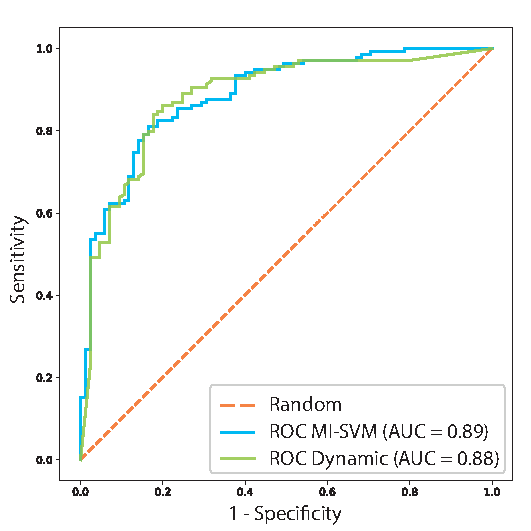
\includegraphics[width=\linewidth]{Figures/Result_Malignancy.pdf}
    \end{subfigure} 
    \begin{subfigure}{.45\linewidth}
        \centering
        \textbf{\ac{lm} \ac{roc} curves}\par
        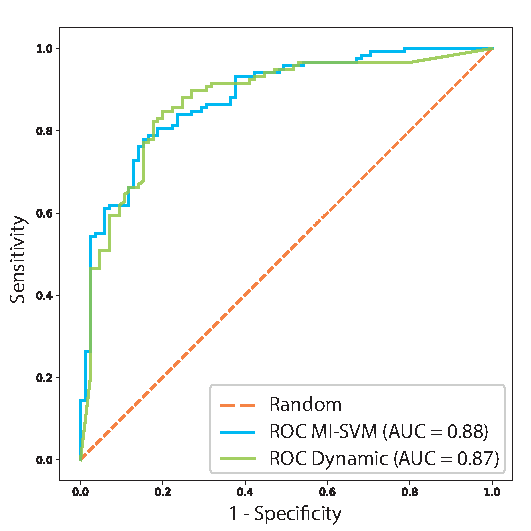
\includegraphics[width=\linewidth]{Figures/Result_LMM.pdf}
    \end{subfigure} 
    
    \caption{On the left, the \ac{roc} curves for Malignancy with the Dynamic and MI-SVM methods. On the right, the \ac{roc} curves for \ac{lm} with the Dynamic and MI-SVM methods.}
    \label{fig:roc_results}
\end{figure}

%=====================================
% DISCUSSION
%=====================================
\section{Conclusions}
\label{sec:conclusions}
This research investigated the classification of malignant tumors and particularly \ac{lm} pathologies at the image-level and at the patient-level. Firstly, at the image-level, an analysis was performed of previous research and proposed methods based on Transfer Learning showing that the Inception-ResNet architecture trained on the ImageNet database is quite relevant for classifying \ac{rcm} images, with a weighted F1 score of 0.83 between benign and malignant labels. Secondly at the patient-level, supervised decision methods were compared to \ac{mil} methods based on feature extraction with the Inception-ResNet architecture. On the first hand, the classification of malignancy over patients achieves a weighted F1-Score of 0.84 with an \ac{auc} score of 0.88 using the supervised method based on a dynamic threshold. It achieves a weighted F1-Score of 0.82 with an \ac{auc} score of 0.89 using the \ac{mil} method based on MI-SVM. On the other hand, the classification of \ac{lm} over patient achieves a weighted F1-Score of 0.83 (Sensitivity 0.88 / Specificity 0.75) with an \ac{auc} score of 0.87 using the supervised method based on a dynamic threshold. It achieves weighted F1-Score of 0.80 (Sensitivity 0.78 / Specificity 0.84) with an \ac{auc} score of 0.88 using the \ac{mil} method based on MI-SVM. Both techniques are relevant compared to the evaluation of dermatologists, reaching 0.80 of sensitivity and 0.81 of specificity with an \ac{auc} score of 0.89. Furthermore, the supervised method based on the dynamic threshold has more sensitivity that can be relevant in the medical context.\par
Further development of these findings should focus on enhancement of the image classification through feature extraction enhancement, in particular by investigation of fine-tuning of the \ac{cnn} architecture. In another step, the patient decision should be improved by working on the score meaning through score calibration methods and by rethinking the way the decision is taken as a result of these.\par

% %%%%%%%%%%%%%%%%%%%%%%%%%%%%%%%%%%%%%%%%%%
\vspace{6pt} 

%%%%%%%%%%%%%%%%%%%%%%%%%%%%%%%%%%%%%%%%%%
\funding{This research was funded by the Conseil Regional de Bourgogne Franche-Comte, France and the European Regional Development Fund (ERDF).}

%%%%%%%%%%%%%%%%%%%%%%%%%%%%%%%%%%%%%%%%%%
\conflictsofinterest{The authors declare no conflict of interest.} 

%%%%%%%%%%%%%%%%%%%%%%%%%%%%%%%%%%%%%%%%%%
\acknowledgments{We thank Dr. Perrot and Dr. Cinotti for their work on the data and the permission granted to exploit it.\par}

%%%%%%%%%%%%%%%%%%%%%%%%%%%%%%%%%%%%%%%%%%
%% optional
\abbreviations{The following abbreviations are used in this manuscript:\\

\noindent 
\begin{tabular}{@{}ll}
\acs{auc}   & \Acl{auc}\\
\acs{bcc}   & \Acl{bcc}\\
\acs{cart}  & \Acl{cart}\\
\acs{cnn}   & \Acl{cnn}\\
\acs{dej}   & \Acl{dej}\\
\acs{ert}   & \Acl{ert}\\
\acs{ggd}   & \Acl{ggd}\\
\acs{glh}   & \Acl{glh}\\
\acs{glcm}  & \Acl{glcm}\\
\acs{lm}    & \Acl{lm}\\
\acs{mil}   & \Acl{mil}\\
\acs{rcm}   & \Acl{rcm}\\
\acs{roc}   & \Acl{roc}\\
\acs{sil}   & \Acl{sil}\\
\acs{svm}   & \Acl{svm}\\
\end{tabular}}

%=====================================
% References
%=====================================
\reftitle{References}
\externalbibliography{yes}
\bibliography{bibliography}

\end{document}

%%%%%%%%%%%%%%%%%%%%%%%%%%%%%%%%%%%%%%%%%%
%% optional
% \sampleavailability{Samples of the compounds ...... are available from the authors.}

%% for journal Sci
%\reviewreports{\\
%Reviewer 1 comments and authors’ response\\
%Reviewer 2 comments and authors’ response\\
%Reviewer 3 comments and authors’ response
%}

%%%%%%%%%%%%%%%%%%%%%%%%%%%%%%%%%%%%%%%%%%

% \begin{table}[h]
%     \centering
%     \begin{tabular}{lllll|lll}
%                                 &                   & \multicolumn{3}{c}{\textbf{Malignancy - F1-Score}}                    & \multicolumn{3}{c}{\textbf{\ac{lm} - F1-Score}}                       \\ \hline
%     \textbf{Category}           & \textbf{Name}     & \textbf{Weighted}     & \textbf{Benign}       & \textbf{Malignant}    & \textbf{Weighted}     & \textbf{Benign}       & \textbf{Malignant}    \\ \hline
%     \multirow{2}{*}{Decision}   & At Least One      & 0.61$\pm$0.06         & 0.32$\pm$0.07         & 0.79$\pm$0.05         & 0.58$\pm$0.07         & 0.32$\pm$0.07         & 0.76$\pm$0.06         \\ \cline{2-8} 
%                                 & \textbf{Dynamic}  & \textbf{0.84$\pm$0.03}& \textbf{0.78$\pm$0.07}& \textbf{0.87$\pm$0.02}& \textbf{0.83$\pm$0.03}& \textbf{0.79$\pm$0.06}& \textbf{0.86$\pm$0.03}\\ \hline 
%     \multirow{2}{*}{Score}      & Mean              & 0.83$\pm$0.03         & 0.78$\pm$0.08         & 0.87$\pm$0.02         & 0.82$\pm$0.03         & 0.79$\pm$0.07         & 0.85$\pm$0.01         \\ \cline{2-8}
%                                 & Maximum           & 0.76$\pm$0.04         & 0.68$\pm$0.03         & 0.80$\pm$0.05         & 0.74$\pm$0.04         & 0.69$\pm$0.03         & 0.78$\pm$0.06         \\ \hline  
%     \multirow{2}{*}{\ac{mil}}   & \ac{sil}          & 0.70$\pm$0.04         & 0.50$\pm$0.10         & 0.83$\pm$0.03         & 0.68$\pm$0.04         & 0.50$\pm$0.10         & 0.80$\pm$0.04         \\ \cline{2-8} 
%                                 & \textbf{MI-SVM}   & \textbf{0.82$\pm$0.02}& \textbf{0.78$\pm$0.05}& \textbf{0.84$\pm$0.02}& \textbf{0.80$\pm$0.03}& \textbf{0.78$\pm$0.05}& \textbf{0.82$\pm$0.03}\\ \hline 
%     \end{tabular}    
%     \caption{Results from patient-level classification for Malignancy(\ac{lm} and \ac{bcc}) and for \ac{lm} along the different proposed methods from \Cref{sec:patient_decision}. For Malignancy and \ac{lm}, the table provide a weighted average of F1-Score, and individual F1-Score for Benign and Malignant classes.}
%     \label{tab:patient_results}
% \end{table}\par